\documentclass[a4paper, 11pt]{article}
\usepackage[utf8]{inputenc}
\usepackage[english,russian]{babel}
\usepackage[T1, T2A]{fontenc}
\usepackage{graphicx}
\usepackage{multirow}
\usepackage{pgfplots}
\pgfplotsset{compat=1.9}
\usepackage[left = 2cm, right = 2cm, bottom = 2cm, top = 2cm]{geometry}
\usepackage{listings}             % Include the listings-package
\usepgfplotslibrary{groupplots}
\usepackage[top=2cm, left=2cm, right=2cm, left=2cm]{geometry}
\usepackage{amsmath}
\usepackage{threeparttable}
\usepackage[tableposition=top]{caption}
\usepackage{subcaption}
\DeclareCaptionLabelFormat{gostfigure}{Рисунок #2}
\DeclareCaptionLabelFormat{gosttable}{Таблица #2}
\DeclareCaptionLabelSeparator{gost}{~---~}
\captionsetup{labelsep=gost}
\captionsetup[figure]{labelformat=gostfigure}
\captionsetup[table]{labelformat=gosttable}
\renewcommand{\thesubfigure}{\asbuk{subfigure}}
\captionsetup[table]{labelformat=simple, labelsep = endash, justification = raggedright, singlelinecheck = off}
\usepackage{indentfirst}

\graphicspath{{image/}}

\newcommand\tline[2]{$\underset{\text{#1}}{\text{\underline{\hspace{#2}}}}$}

\begin{document}
	\begin{titlepage}
		\centering
		{\fontsize{12pt}{5cm}\selectfont \bfseries Министерство образования и науки Российской Федерации} \\ \vspace{0.5cm}
		{\fontsize{7pt}{5cm}\selectfont ФЕДЕРАЛЬНОЕ ГОСУДАРСТВЕННОЕ АВТОНОМНОЕ ОБРАЗОВАТЕЛЬНОЕ УЧРЕЖДЕНИЕ ВЫСШЕГО ПРОФЕССИОНАЛЬНОГО ОБРАЗОВАНИЯ} \\ 
		\vspace{1cm}
		{\fontsize{12pt}{5cm}\selectfont \bfseries САНКТ-ПЕТЕРБУРГСКИЙ УНИВЕРСИТЕТ ИНФОРМАЦИОННЫХ ТЕХНОЛОГИЙ, МЕХАНИКИ И ОПТИКИ} \\ \vspace{1.5cm}

		{\fontsize{14pt}{5cm}\selectfont Кафедра \hspace{1cm} \underline{Систем Управления и Информатики}  \hspace{1cm} Группа \underline{Р3340}} \\ 
		\vspace{2cm}

		{\fontsize{20pt}{5cm}\selectfont \bfseries Лабораторная работа №8} \\
		{\fontsize{20pt}{5cm}\selectfont \bfseries “Экспериментальное построение областей устойчивости линейной системы на плоскости двух параметров”} \\
		{\fontsize{14pt}{5cm}\selectfont Вариант - 7} \\
		\vspace{1.5cm}

		\flushleft

		{Выполнил \hspace{2cm} \tline{(фамилия, и.о.)}{9cm} (подпись)} \\
		\vspace{2cm}

		{Проверил \hspace{2cm} \tline{(фамилия, и.о.)}{9cm} (подпись)} \\
		\vspace{5cm}

		"\underline{\hspace{0.7cm}}"\hspace{0.2cm}\underline{\hspace{2cm}}\hspace{0.2cm}20\underline{\hspace{0.7cm}}г. \hspace{2cm} Санкт-Петербург, \hspace{2cm} 20\underline{\hspace{0.7cm}}г. \\ \vspace{1cm}

		Работа выполнена с оценкой \hspace{1cm} \underline{\hspace{8cm}} \\ 
		\vspace{1cm}
		Дата защиты "\underline{\hspace{0.7cm}}"\hspace{0.2cm}\underline{\hspace{2cm}}\hspace{0.2cm}20\underline{\hspace{0.7cm}}г.

\end{titlepage}

\begin{center}
\section*{Задание}
\end{center}

\subsection*{Цель работы} 
Ознакомление с экспериментальными методами построения областей устойчивости линейных динамических систем и изучение влияния на устойчивость системы ее параметров. В работе будет изучаться система третьего порядка, типичная для широкого класса электромеханических объектов управления. При зафиксированной постоянной времени $T_1$ и изменении параметров $T_2$ и $k$ ставится цель определить границу устойчивости на основе критерия Гурвица.

\subsection*{Исходные данные}
\par
$T_1 = 2 c$
\par
На рисунке 1 изображена структурная схема моделируемой системы:
\begin{figure}[h]
\center{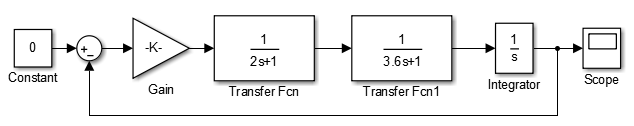
\includegraphics[width=0.75\linewidth]{model.png}}
\caption{Структурная схема моделируемой системы}
\label{ris:image}
\end{figure}

\newpage
\begin{center}
\section{Исследование устойчивости при варьировании параметров $k$ и $T_2$}
\end{center}
\par
\pgfplotsset{
every axis plot post/.append style={
	mark= ,
	every mark/.append style={solid},
	every axis title/.style={at={(0.5,0)},anchor=north,yshift=-0.1}
	}}
На рисунке 2 изображён график выходного сигнала системы, имеющий устойчивый характер:
\begin{figure}[h!]
\centering
\begin{tikzpicture}
\begin{axis}[
	xmin = 0,
	xmax = 30,
	xlabel = {\Large{$t,c$}},
	ylabel = {\Large{$y$}},
	width = 250,
	height = 200,
	grid = both,
]

\addplot[line width = 2] table [x=t, y=y] 
              {data/ust.txt};

\end{axis}
\end{tikzpicture}
\caption{Результаты моделирования при $k=1$, $T_2=0.1$}
\end{figure}

На рисунке 3 изображён график выходного сигнала системы при устойчивости нейтрального типа:
\begin{figure}[h!]
\centering
\begin{tikzpicture}
\begin{axis}[
	xmin = 0,
	xmax = 30,
	xlabel = {\Large{$t,c$}},
	ylabel = {\Large{$y$}},
	width = 250,
	height = 200,
	grid = both,
]

\addplot[line width = 2] table [x=t, y=y] 
              {data/neitral.txt};

\end{axis}
\end{tikzpicture}
\caption{Результаты моделирования при $k=1$, $T_2=0.1$}
\end{figure}

На рисунке 4 изображён график выходного сигнала системы при устойчивости колебательного типа:
\begin{figure}[h!]
\centering
\begin{tikzpicture}
\begin{axis}[
	xmin = 0,
	xmax = 30,
	xlabel = {\Large{$t,c$}},
	ylabel = {\Large{$y$}},
	width = 250,
	height = 200,
	grid = both,
]

\addplot[line width = 2] table [x=t, y=y] 
              {data/koleb.txt};

\end{axis}
\end{tikzpicture}
\caption{Результаты моделирования при $k=10.5$, $T_2=0.1$}
\end{figure}

\newpage
На рисунке 5 график выходного сигнала системы представлен при типичной неустойчивости:
\begin{figure}[h!]
\centering
\begin{tikzpicture}
\begin{axis}[
	xmin = 0,
	xmax = 30,
	xlabel = {\Large{$t,c$}},
	ylabel = {\Large{$y$}},
	width = 250,
	height = 200,
	grid = both,
]

\addplot[line width = 2] table [x=t, y=y] 
              {data/neust.txt};

\end{axis}
\end{tikzpicture}
\caption{Результаты моделирования при $k=15$, $T_2=0.1$}
\end{figure}

\newpage
\begin{center}
\section{Теоретический расчёт границы устойчивости с использованием критерия Гурвица}
\end{center}

Найдём  передаточную функцию системы:
\begin{equation}
W(s)=\frac{k}{2T_2s^3+(2+T_2)s^2+s+k}
\end{equation}
\par
Составим матрицу Гурвица:
\begin{equation}
\begin{bmatrix}
(2+T_2) & k & 0\\
2T_2 & 1 & 0\\
0 & (2+T_2) & k
\end{bmatrix}
\end{equation}

Запишем критерии колебательной устойчивости:
\begin{equation}
\begin{cases}
	2+T_2 > 0 \\
	k = \displaystyle{\frac{2+T_2}{2T_2}} \\
	k > 0
\end{cases}
\end{equation}
\par
А также запишем критерии для устойчивости нейтрального типа:
\begin{equation}
k=0
\end{equation}
\par
Таким образом, меняя параметр $T_2$ можно получить необходимую границу устойчивости.
На рисунке 6 представлены графики экспериментальной и теоретической границ устойчивости. 
\par
При экспериментальном подборе значений коэффициента $k$ для разных значений $T_2$ была получена таблица значений для постоения экспериментальной границы устойчивости. Экспериментальные и теоретические точки представлены в таблице 1.

\begin{table}[h!]
\centering
\begin{threeparttable}
\caption{Данные для определения границы устойчивости}\label{tab:perflogcross}
\begin{tabular}{|c|c|c|c|c|c|c|c|c|c|c|c|}
\hline
$T_2,c$ & 0.1 & 0.5 & 1 & 1.5 & 2 & 2.5 & 3 & 3.5 & 4 & 4.5 & 5\\
\cline{1-12}
$k_{expr}$ & 10.55 & 2.5 & 1.5 & 1.166 & 1 & 0.9 & 0.83 & 0.79 & 0.75 & 0.72 & 0.7\\
\cline{1-12}
$k_{anal}$ & 10.5 & 2.5 & 1.5 & 1.166 & 1 & 0.9 & 0.83 & 0.79 & 0.75 & 0.72 & 0.7\\
\hline

\end{tabular}
\end{threeparttable}
\end{table}

\begin{figure}[h!]
\centering
\begin{tikzpicture}
\begin{axis}[
	xmin = 0,
	xlabel = {\Large{$T_2,c$}},
	ylabel = {\Large{$k$}},
	width = 250,
	height = 200,
	grid = both,
]

\addplot[line width = 2] table [x=t, y=y] 
              {data/data.txt};
\addplot[line width = 2, loosely dashed, draw = red]table [x=t, y=y]
				{data/data_expr.txt};
\addplot[line width = 2] {0};

\legend{
	$k(T_2)_{anal}$,
	$k(T_2)_{expr}$
	}

\end{axis}
\end{tikzpicture}
\caption{Полученная теоретически граница устойчивости}
\end{figure}

\par
Как видно на рисунке 6, полученные графики идентичны, за исключением точки $(0.1;10.55)$.
\newpage
\begin{center}
\section*{Выводы}
\end{center}
\par
В данной лабораторной работе я изучил систему третьего порядка на предмет устойчивости. Для определения границы устойчивости я выбрал 2 параметра($T_2$ и $k$), а затем путём их варьирования на основе критерия Гурвица для системы третьего порядка получил массив значений для построения границы устойчивости. На основе полученных данных можно сказать, что график устойчивости представляет собой ветвь гиперболы, ограниченную снизу прямой $k=0$.
\end{document}
